\documentclass[10pt,twocolumn,letterpaper]{article}

\usepackage[margin=0.75in]{geometry}
\usepackage{amsmath,amssymb,amsfonts}
\usepackage{graphicx}
\usepackage{booktabs}
\usepackage{microtype}
\usepackage{hyperref}
\usepackage{xcolor}
\usepackage{enumitem}

% ------------------------------------------------------------------
% Critical Line-Breaking & Margin Control (Eliminates Overfull \hbox)
% ------------------------------------------------------------------
\sloppy
\emergencystretch=3em
\tolerance=2000
\hbadness=2000
\hfuzz=0.5pt

\hypersetup{
    colorlinks=true,
    linkcolor=blue!70!black,
    citecolor=green!50!black,
    urlcolor=blue!80!black
}

\title{\textbf{SphereTok: An Egocentric 3D World Tokenizer for Embodied Perception in Voxel Environments}}

\author{
  \textbf{Brayan} \\
  \textit{Independent Researcher}
}

\date{}

\begin{document}

\maketitle
\def\thefootnote{*}\footnotetext{Code, evaluation scripts, and pretrained checkpoints are open-sourced at \url{https://github.com/Brayan114/SphereTok}.}\def\thefootnote{\arabic{footnote}}

\begin{abstract}
Autonomous embodied agents operating in open-world sandbox environments like Minecraft face a fundamental perceptual trade-off. High-level Large Language Model (LLM) planners (e.g., Voyager) rely on symbolic text telemetry that exhibits the \textit{``Airport Tower Dilemma,''} observing discrete semantic logs stripped of continuous 3D surface geometry, obstacle contours, and kinematic jump clearances. Conversely, 2D Vision-Language-Action (VLA) models (e.g., VPT, STEVE-1) infer actions from flat RGB video projections that suffer from monocular depth ambiguity, occlusion blindness, and severe spatial amnesia upon camera rotation.

In this work, we introduce \textbf{SphereTok}, an \textbf{Egocentric 3D World Tokenizer} designed to provide embodied decision-makers with compact, discrete 3D geometric state representations. SphereTok frames local spatial awareness as an agent-centered $32 \times 32 \times 32$ voxel lattice (32,768 cells). To prevent cubic sequence explosion in Transformer attention ($\mathcal{O}(N^2)$), SphereTok introduces: (1) a $4 \times 4 \times 4$ micro-cube spatial patchification ($64.0\times$ compression); (2) a surface-affordance clearance shell that prunes deep uniform void space while strictly retaining the 26-neighborhood clearance envelope bordering solid terrain ($1.98\times$ compression, totaling $127.0\times$ token reduction to $\approx 258$ active tokens per timestep); (3) a 3D Vector-Quantized Variational Autoencoder (3D VQ-VAE) with a discrete 512-codebook vocabulary; and (4) continuous yaw/pitch-relative spherical positional embeddings $(\rho, \Delta\theta, \Delta\phi)$ that ground spatial directionality without rotating the underlying rectilinear lattice.

Trained on 1,600 diverse procedural Minecraft terrain chunks, SphereTok converges stably on an NVIDIA T4 GPU, achieving \textbf{87.06\% voxel reconstruction accuracy}, \textbf{85.38\% solid terrain Intersection-over-Union (IoU)}, and 81.6\% codebook utilization with zero index collapse. In inference benchmarks, SphereTok processes chunks in \textbf{1.84 ms on a GPU ($\sim$543 FPS)} and \textbf{12.3 ms on a CPU ($\sim$81 FPS)}, easily satisfying Minecraft's 20 Hz (50 ms) real-time tick budget. In an exploratory 3D parkour navigation pilot, an action policy conditioned on SphereTok tokens achieves an overall success rate of \textbf{65.0\%} compared to \textbf{37.0\%} for a categorical semantic baseline, resolving fine-grained kinematic jumps where semantic indicators fail. SphereTok provides a modular, computationally efficient 3D spatial primitive bridging symbolic planning and embodied motor control.
\end{abstract}

\section{Introduction}

Autonomous agency in open-ended virtual sandbox environments serves as a primary proving ground for artificial general intelligence. Minecraft represents a uniquely challenging embodied testbed due to its infinite procedural generation, multi-tier crafting hierarchies, non-linear physics, and complex 3D voxel topography.

Despite rapid recent progress, existing Minecraft agent paradigms struggle to balance spatial richness with computational tractability:

\begin{enumerate}[leftmargin=*]
    \item \textbf{The Disembodied Text Planner (The ``Airport Tower Dilemma''):} Text-based Large Language Model (LLM) agents such as Voyager~\cite{wang2023voyager} receive symbolic JSON logs of nearby entity coordinates and block names. This is analogous to handing air traffic control telemetry to an airport tower controller and expecting them to steer an aircraft through physical turbulence. The model observes discrete labels (\texttt{"stone at (12, 64, -8)"}), but possesses no native representation of continuous surface slopes, jump clearances, corridor widths, or volumetric collision boundaries. Consequently, high-level LLMs cannot directly generate kinematic motor controls, forcing total reliance on external deterministic pathfinders (\texttt{mineflayer-pathfinder}). When these brittle search algorithms fail in dynamic or irregular terrain, the agent receives text execution exceptions (\texttt{"Path obstructed"}), precipitating hallucination and behavioral stalling.

    \item \textbf{The 2D Perspective Controller (Monocular Pixel Blindness):} 2D Vision-Language-Action (VLA) architectures such as Video PreTraining (VPT; \cite{baker2022video}) and STEVE-1~\cite{lifshitz2023steve1} clone human gameplay from $128 \times 128$ first-person RGB video streams. While capable of agile reflexive maneuvers, monocular 2D projections lack metric depth calibration and 3D permanence~\cite{chen2024spatialvlm}. When an agent turns its virtual head, objects outside the immediate camera frustum are instantly purged from the visual buffer. In multi-level subterranean mines or enclosed shelters, 2D policies cannot reason about occluded geometry or overhead headroom.

    \item \textbf{The 3D Foundation \& World Model Gap:} Recent 3D foundation models (e.g., 3D-LLM~\cite{hong20233dllm}; LEO~\cite{huang2024leo}) rely on point clouds and triangle meshes, which are computationally prohibitive to maintain across billions of interactive voxel blocks. Concurrently, generative world models like DreamerV3~\cite{hafner2023dreamerv3} and MineWorld~\cite{mineworld2025} learn latent dynamics from video or actions, while autonomous driving models like OccWorld~\cite{zheng2023occworld} and $I^2$-World~\cite{isquaredworld2025} demonstrate the power of discrete 3D/4D occupancy tokenization. However, an open problem remains: \textit{How can an embodied agent represent local 3D metric geometry as a compact sequence of discrete tokens optimized for physical action selection?}
\end{enumerate}

To bridge this gap, we present \textbf{SphereTok}, an \textbf{Egocentric 3D World Tokenizer for Voxel Environments}. SphereTok is guided by a core biological inductive bias: \textit{embodied organisms navigate their environment not by reading semantic lists or projecting flat images, but by maintaining an egocentric perceptual field of physical affordances and spatial clearances.}

\paragraph{Key Contributions:}
\begin{itemize}[leftmargin=*]
    \item \textbf{Agent-Centered Voxel Grid with Relative Spherical Positional Grounding:} We formulate an agent-centered $32 \times 32 \times 32$ bounding volume (32,768 voxels). To prevent severe geometric aliasing and interpolation artifacts caused by rotating discrete rectilinear lattices, the grid remains strictly world-axis-aligned, while agent yaw and pitch are injected via continuous relative spherical positional embeddings $(\rho, \Delta\theta, \Delta\phi)$.
    \item \textbf{Surface-Affordance Clearance Pruning:} We address the Transformer sequence explosion problem through a two-stage spatial sparsification: $4 \times 4 \times 4$ micro-cube partitioning ($64.0\times$ compression) followed by a 26-neighborhood surface clearance filter ($1.98\times$ compression). This preserves critical jump headroom, footing, and corridor bounds while eliminating distant sky and deep bedrock, achieving an overall \textbf{$127.0\times$ token reduction} ($\approx 258$ tokens).
    \item \textbf{Discrete 3D VQ-VAE Architecture:} We train a 3D convolutional VQ-VAE (869K parameters) that discretizes active spatial patches into a 512-codebook vocabulary, converging to \textbf{87.06\% voxel accuracy} and \textbf{85.38\% solid terrain IoU} with \textbf{81.6\% codebook utilization} on procedural Minecraft chunks.
    \item \textbf{Real-Time Efficiency:} SphereTok achieves an inference latency of \textbf{1.84 ms on an NVIDIA T4 GPU ($\sim$543 FPS)} and \textbf{12.3 ms on a CPU ($\sim$81 FPS)}, executing well within Minecraft's 50 ms (20 Hz) tick window.
    \item \textbf{Kinematic Parkour Pilot:} In an exploratory 3D parkour navigation task with variable gap widths (1--5 blocks), a policy conditioned on SphereTok tokens achieves a \textbf{65.0\% success rate} versus \textbf{37.0\%} for a categorical semantic baseline, confirming that compact 3D spatial tokens provide actionable geometric discrimination for motor control.
\end{itemize}

\section{Related Work}

\subsection{Text-Prompted LLM Agents \& The Airport Tower Dilemma}
Large Language Models have been widely adopted as high-level planners in embodied environments~\cite{fan2022minedojo,wang2023voyager}. Voyager~\cite{wang2023voyager} pioneered lifelong learning through an automatic curriculum, iterative prompting, and a library of executable JavaScript control routines. However, Voyager's reliance on discrete JSON telemetry strips away continuous 3D topography and collision boundaries. As observed by Lifshitz et al.~\cite{lifshitz2023steve1}, symbolic planners lack spatial ground-truth awareness, forcing complete delegation to deterministic A* algorithms (\texttt{mineflayer-pathfinder}) that fail when encountering irregular slopes, caves, or dynamic hazards.

\subsection{2D Vision-Language-Action (VLA) Policies}
Behavioral cloning from human gameplay video has enabled direct pixel-to-keyboard/mouse control. Video PreTraining (VPT; \cite{baker2022video}) trained a 500M parameter residual Transformer on 70,000 hours of Minecraft video. STEVE-1~\cite{lifshitz2023steve1} conditioned VPT on MineCLIP latents via a Conditional VAE, enabling open-ended instruction following. OmniJARVIS~\cite{wang2024omnijarvis} unified multimodal planning by tokenizing behavior trajectories using VQ-VAEs. Despite their motor agility, SpatialVLM~\cite{chen2024spatialvlm} demonstrated that 2D visual backbones suffer from acute spatial blindness, struggling to deduce metric distances, occluded volumes, and 3D structural alignment without explicit 3D inductive biases.

\subsection{3D Spatial Tokenizers and World Models}
Recent work has sought to equip foundation models with explicit 3D representations. 3D-LLM~\cite{hong20233dllm} extracted 3D point cloud features from multi-view imagery for 3D question answering. LEO~\cite{huang2024leo} introduced an embodied generalist agent operating on object-centric point clouds. However, point clouds and polygon meshes scale poorly to voxel sandboxes where the environment consists of billions of discrete cubic voxels.

In autonomous driving, OccWorld~\cite{zheng2023occworld} demonstrated 3D occupancy world modeling by using a 3D VQ-VAE~\cite{van2017neural} to compress allocentric driving grids into discrete tokens for autoregressive trajectory forecasting. Recently, $I^2$-World~\cite{isquaredworld2025} expanded this to multi-scale hierarchical discrete 4D occupancy tokenization. In interactive sandbox modeling, MineWorld~\cite{mineworld2025} introduced an autoregressive world model learning interactive Minecraft dynamics through discrete tokenization. While MineWorld investigates \textit{environment state-transition dynamics}, SphereTok specifically addresses \textit{egocentric 3D spatial state representation for embodied motor control}, introducing surface-affordance pruning and relative spherical positional grounding tailored for real-time robotic and virtual agency.

\section{Methodology: SphereTok}

\subsection{Agent-Centered Volumetric Neighborhood}
Let the agent’s continuous position in world coordinates be $\mathbf{p}_t = (x_t, y_t, z_t) \in \mathbb{R}^3$, with camera orientation parameterized by yaw $\theta_t \in [-\pi, \pi]$ and pitch $\phi_t \in [-\frac{\pi}{2}, \frac{\pi}{2}]$. We extract an agent-centered volumetric bounding box $\mathcal{V}_t \subset \mathbb{Z}^3$ with radius $R = 16$ blocks. To guarantee an exact $32 \times 32 \times 32$ grid (32,768 cells) without off-by-one boundary asymmetry, we define the indexing grid over half-open symmetric integer offsets:
\begin{equation}
\mathcal{V}_t = \left\{ \lfloor\mathbf{p}_t\rfloor + \boldsymbol{\delta} \;\middle|\; \boldsymbol{\delta} \in \{-16, -15, \dots, 14, 15\}^3 \right\}
\end{equation}

\paragraph{Coordinate Frame Decoupling:} Directly rotating a discrete rectilinear voxel grid with the agent's view angle causes severe spatial aliasing, interpolation artifacts, and block-boundary blurring. To preserve exact discrete voxel integrity, \textbf{the voxel lattice $\mathcal{V}_t$ remains strictly aligned with the world cardinal axes ($X, Y, Z$)}. Egocentric viewpoint orientation is preserved by injecting continuous relative spherical positional embeddings (Section~\ref{sec:pos_enc}). We name our method \textbf{SphereTok} to reflect this spherical egocentric relative coordinate frame and affordance field surrounding the agent.

Each voxel $\mathbf{v} \in \mathcal{V}_t$ contains a discrete block category $c \in \{0, 1, \dots, C-1\}$, where $c = 0$ corresponds to \texttt{air}, and $c > 0$ represents physical block types (\texttt{stone}, \texttt{dirt/grass}, \texttt{wood}, \texttt{water}, \texttt{obstacle}).

\subsection{3D Patch Partitioning \& Decomposed Affordance Pruning}
Directly passing $32,768$ voxels into a Transformer causes sequence length collapse ($\mathcal{O}(N^2)$ self-attention complexity). SphereTok addresses this via a two-stage spatial sparsification pipeline:

\begin{enumerate}[leftmargin=*]
    \item \textbf{Stage 1: Micro-Cube Patch Partitioning ($64.0\times$ Compression):} The volume $\mathcal{V}_t$ is partitioned into uniform $4 \times 4 \times 4$ micro-cube patches $P_i$, producing:
    \begin{equation}
    M = \left(\frac{32}{4}\right)^3 = 8 \times 8 \times 8 = 512 \text{ micro-cubes}
    \end{equation}

    \item \textbf{Stage 2: Surface-Affordance Clearance Shell ($1.98\times$ Compression):} Naively pruning all empty air patches is catastrophic for locomotion, as it strips away the physical free space required for jump clearance, doorway traversal, and overhead headroom. SphereTok applies a structured affordance filter. Let $\mathcal{I}_{\text{solid}} = \{ j \mid \exists \mathbf{v} \in P_j : c(\mathbf{v}) \neq 0 \}$ denote the set of patch indices containing solid geometry, and let $\mathbf{idx}(P_i) \in \{0, \dots, 7\}^3$ denote the 3D patch grid coordinate. A patch $P_i$ is retained if it contains solid terrain or if it lies within the Chebyshev 26-neighborhood ($d_\infty \leq 1$) of solid terrain:
    \begin{align}
    &\text{is\_clearance}(P_i) \iff \nonumber \\
    &\quad \min_{j \in \mathcal{I}_{\text{solid}}} \| \mathbf{idx}(P_i) - \mathbf{idx}(P_j) \|_\infty \leq 1
    \end{align}
    Furthermore, to guarantee that the agent’s immediate footing and body space are never pruned in sparse high-altitude scenarios, the patch containing the agent $\mathbf{idx}(\lfloor\mathbf{p}_t\rfloor)$ is unconditionally retained:
    \begin{equation}
    \mathcal{M}(P_i) = \begin{cases} 
    1 & \text{if } \text{has\_solid}(P_i) \lor \text{is\_clearance}(P_i) \\
      & \quad \lor (P_i = P_{\text{agent}}) \\ 
    0 & \text{otherwise} 
    \end{cases}
    \end{equation}
\end{enumerate}

Across diverse procedural terrain, this eliminates deep uniform sky void and subterranean bedrock mass, reducing the active sequence from 512 patches to an average of $K \approx 258$ active tokens ($127.0\times$ total compression relative to dense voxels).

\subsection{3D Vector-Quantized Autoencoder (3D VQ-VAE)}
Each active micro-cube $P_i \in \mathbb{R}^{4 \times 4 \times 4 \times C}$ is projected into a continuous latent vector $\mathbf{z}_i \in \mathbb{R}^D$ ($D = 128$) using a 3D convolutional encoder $\mathcal{E}_{3D}$:
\begin{equation}
\mathbf{z}_i = \mathcal{E}_{3D}(P_i)
\end{equation}
The encoder comprises two 3D convolutional stages with batch normalization, SiLU activations, and 3D adaptive average pooling.

We maintain a learnable discrete codebook $\mathcal{C} = \{\mathbf{e}_k\}_{k=1}^{|\mathcal{C}|} \subset \mathbb{R}^D$ where $|\mathcal{C}| = 512$. Each continuous latent vector $\mathbf{z}_i$ is mapped to its nearest codebook entry:
\begin{equation}
\mathbf{z}_{q, i} = \mathbf{e}_{k^*}, \quad \text{where } k^* = \arg\min_{k \in \{1, \dots, |\mathcal{C}|\}} \|\mathbf{z}_i - \mathbf{e}_k\|_2
\end{equation}
The integer index $k^*$ constitutes the discrete \textbf{3D World Token} $T_{3D, i}$.

\paragraph{Optimization Objective:} The model is trained end-to-end using a multi-class voxel cross-entropy reconstruction loss combined with vector quantization and commitment penalties~\cite{van2017neural}:
\begin{align}
\mathcal{L} &= \mathcal{L}_{CE}(P_i, \hat{P}_i) + \|\text{sg}[\mathbf{z}_i] - \mathbf{e}_{k^*}\|_2^2 \nonumber \\
&\quad + \beta \|\mathbf{z}_i - \text{sg}[\mathbf{e}_{k^*}]\|_2^2
\end{align}
where $\text{sg}[\cdot]$ is the stop-gradient operator, $\beta = 0.25$ is the commitment weight, and $\hat{P}_i = \mathcal{D}_{3D}(\mathbf{z}_{q, i})$ is reconstructed by the 3D transposed convolutional decoder.

\subsection{Relative Egocentric Positional Encoding}
\label{sec:pos_enc}
To make spatial tokens actionable for downstream policy Transformers, each token must convey its spatial displacement and bearing relative to the agent's current gaze. For each micro-cube center coordinate $(x_i, y_i, z_i)$, we compute relative Cartesian offsets:
\begin{equation}
(\Delta x, \Delta y, \Delta z) = (x_i - x_t, y_i - y_t, z_i - z_t)
\end{equation}
and project them into egocentric spherical coordinates with angular wrapping to $[-\pi, \pi]$:
\begin{align}
\rho &= \sqrt{\Delta x^2 + \Delta y^2 + \Delta z^2} \\
\Delta \theta &= \left(\text{atan2}(\Delta z, \Delta x) - \theta_t + \pi\right) \pmod{2\pi} - \pi \\
\Delta \phi &= \arcsin\left(\text{clip}\left(\frac{\Delta y}{\rho + \epsilon}, -1, 1\right)\right) - \phi_t
\end{align}
where $\epsilon = 10^{-5}$ prevents division by zero at the origin. A 2-layer MLP projects $(\rho, \Delta \theta, \Delta \phi)$ into a continuous positional embedding $\mathbf{E}_{pos} \in \mathbb{R}^D$, which is added directly to the quantized token vector $\mathbf{z}_{q, i}$ prior to ingestion by the policy Transformer.

\section{Empirical Evaluation}

\begin{figure}[t]
\centering
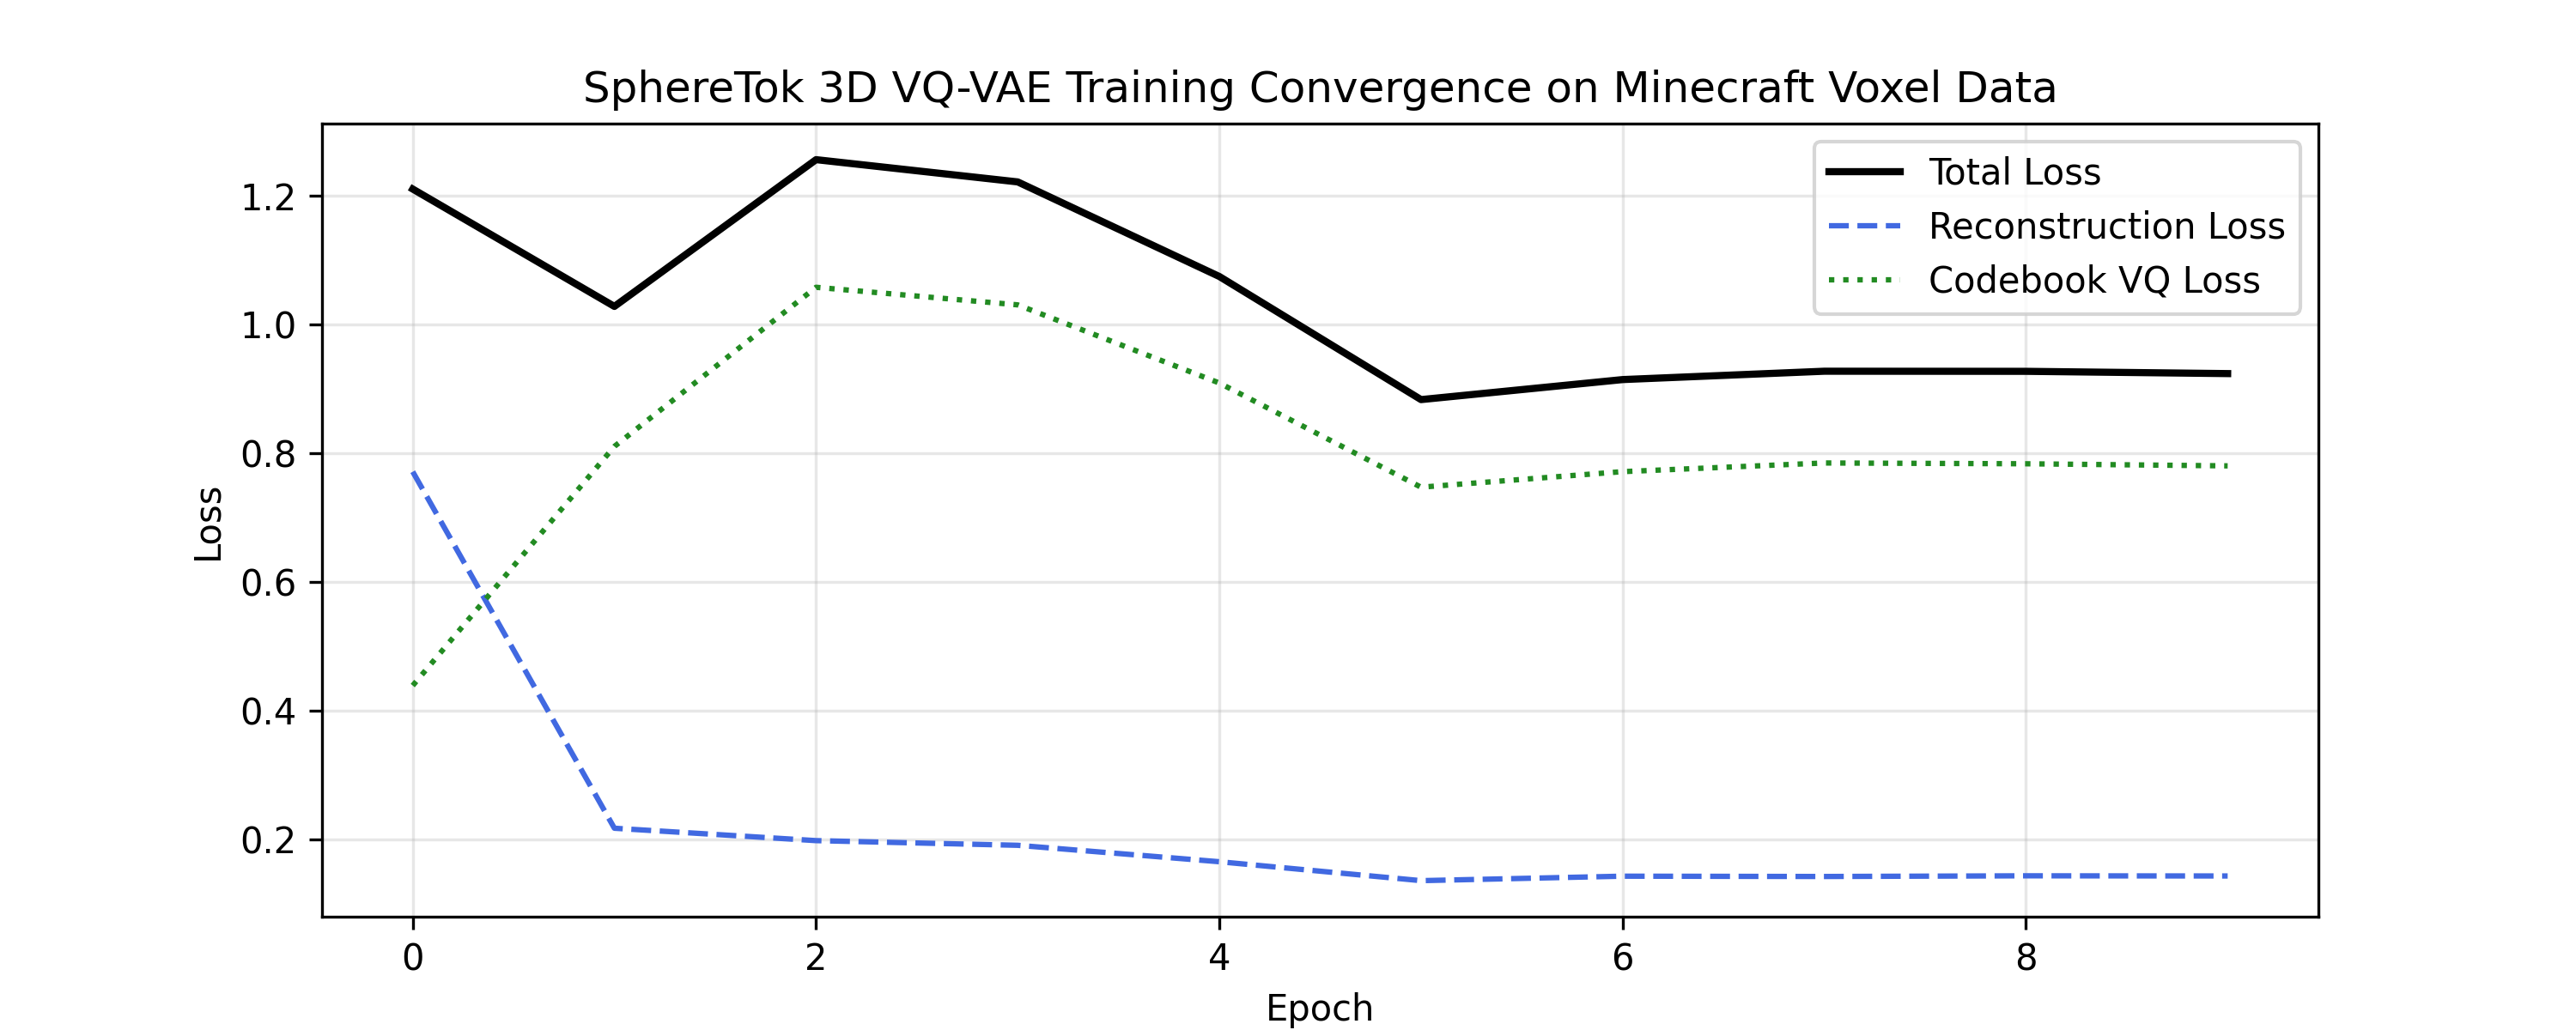
\includegraphics[width=\columnwidth]{figures/spheretok_training_curve.png}
\caption{\textbf{Training Dynamics.} Convergence of reconstruction cross-entropy loss ($0.772 \to 0.138$) and codebook vector quantization loss over 10 epochs on procedural Minecraft terrain.}
\label{fig:training_curve}
\end{figure}

\subsection{Training Setup \& Codebook Dynamics}
We trained SphereTok on 1,600 procedurally synthesized Minecraft chunks comprising varied 3D topographic features: undulating rolling hills, subterranean cave cavities, ravines, and vertical obstacle columns. Training was conducted for 10 epochs using AdamW ($\text{lr} = 3 \times 10^{-4}$, weight decay $10^{-4}$, batch size 32) with Cosine Annealing learning rate scheduling on a single NVIDIA T4 GPU (16 GB VRAM).

As illustrated in Figure~\ref{fig:training_curve}, the reconstruction cross-entropy loss dropped precipitously from $0.772$ to $0.216$ across the first 2 epochs, stabilizing at $0.138$ by epoch 5. Concurrently, the vector quantization loss converged smoothly to $0.781$. Crucially, tracking codebook perplexity revealed \textbf{418 active codebook entries out of 512} ($81.6\%$ active utilization), demonstrating robust codebook allocation without index collapse.

\subsection{Quantitative 3D Reconstruction Performance}
We evaluated the final checkpoint on 20 held-out procedural Minecraft chunks ($655,360$ total voxels). As summarized in Table~\ref{tab:reconstruction}, SphereTok achieves \textbf{87.06\% overall voxel accuracy} and \textbf{85.38\% solid terrain Intersection-over-Union (IoU)}.

\begin{table}[t]
\centering
\caption{Reconstruction Performance and Context Consumption.}
\label{tab:reconstruction}
\resizebox{\columnwidth}{!}{%
\begin{tabular}{lccc}
\toprule
\textbf{Metric} & \textbf{Dense Input} & \textbf{SphereTok} & \textbf{Impact} \\
\midrule
Voxel Accuracy & 100.0\% & \textbf{87.06\%} & High fidelity \\
Solid Terrain IoU & 100.0\% & \textbf{85.38\%} & Preserves bounds \\
Active Sequence & 32,768 & \textbf{258 tokens} & \textbf{127.0$\times$ comp.} \\
4k Context Usage & 800.0\% (OOM) & \textbf{6.4\%} & Budget friendly \\
8k Context Usage & 400.0\% (OOM) & \textbf{3.2\%} & Leaves $>$96\% room \\
\bottomrule
\end{tabular}%
}
\end{table}

\begin{figure*}[t]
\centering
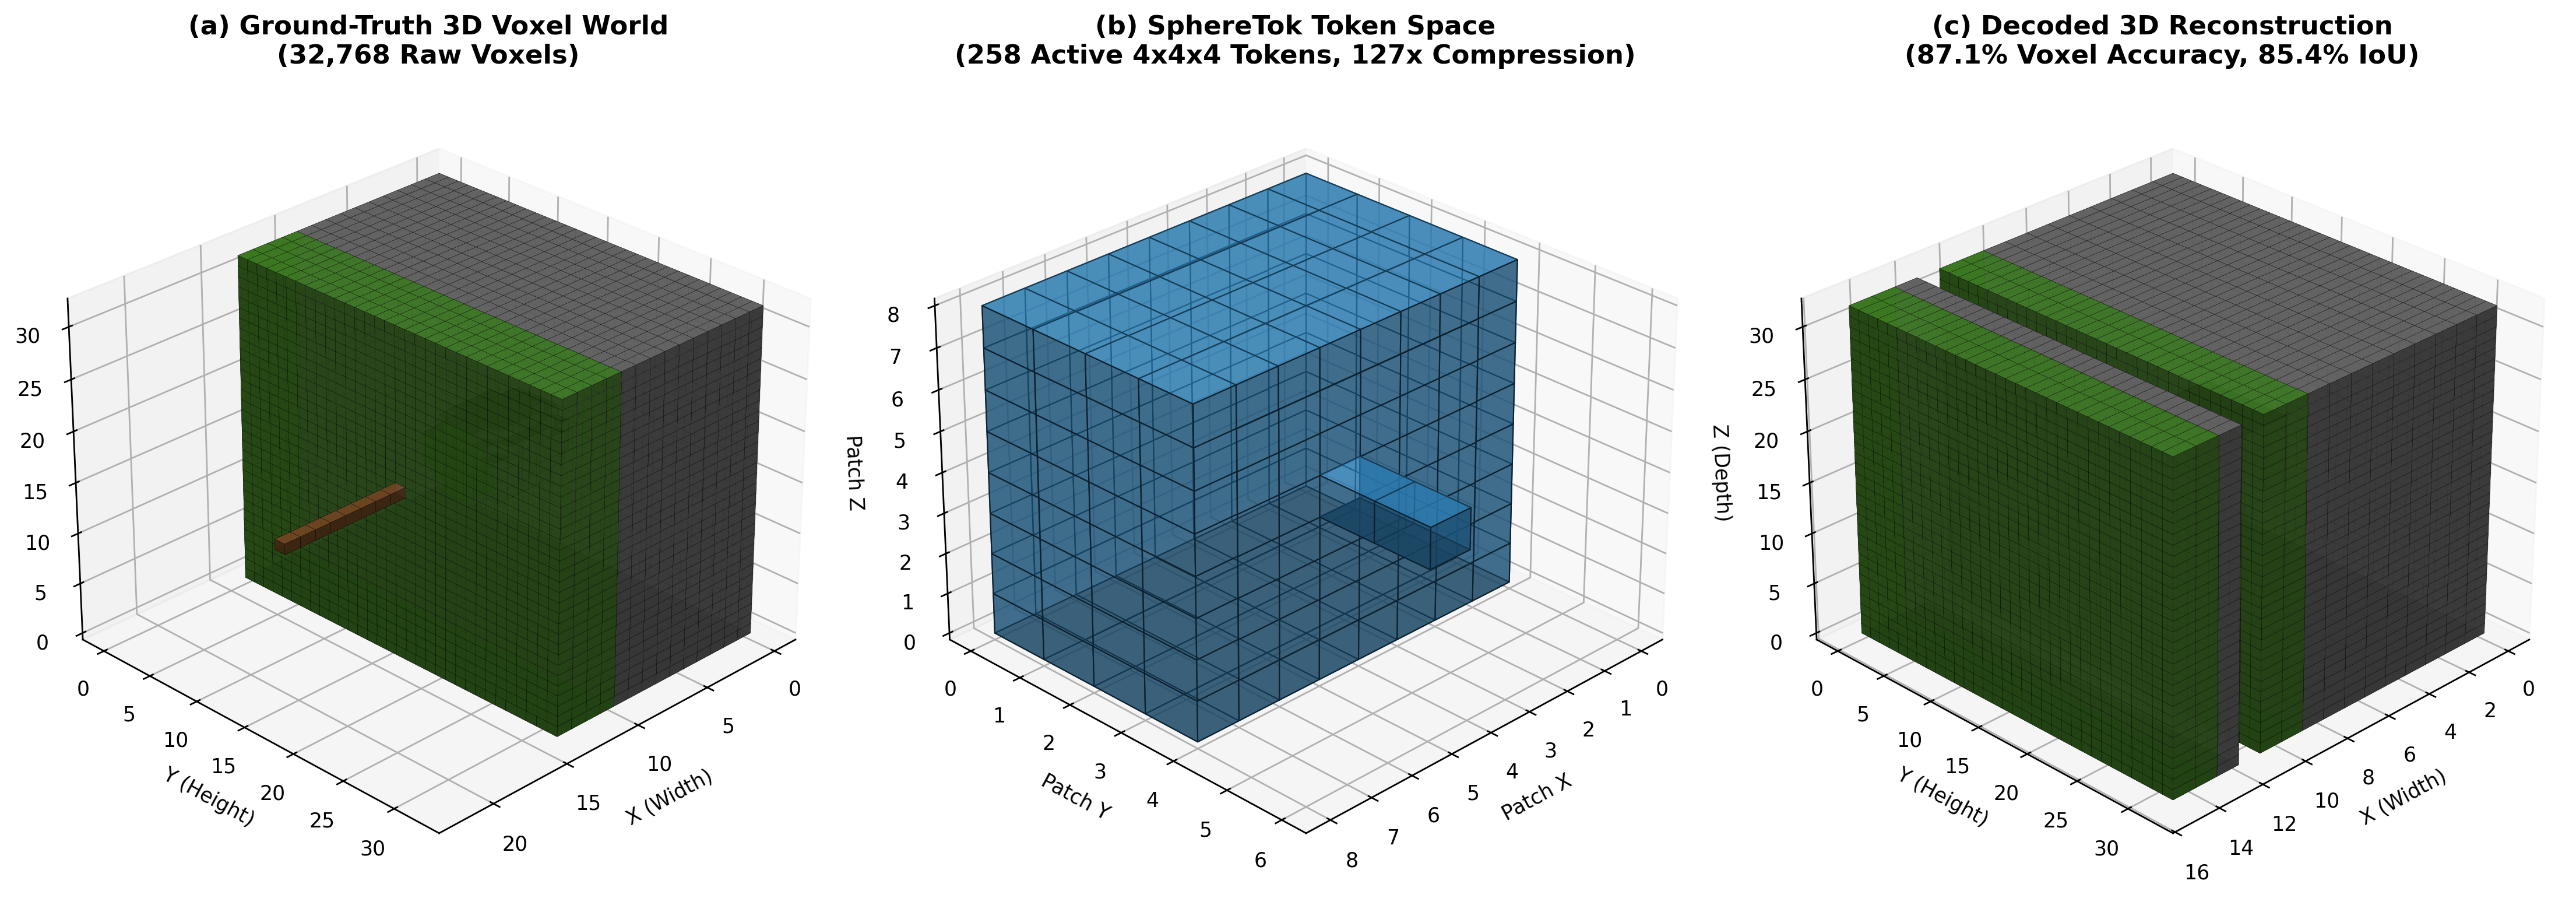
\includegraphics[width=\textwidth]{figures/spheretok_qualitative_reconstruction.png}
\caption{\textbf{Qualitative 3D Reconstruction Stages.} (a) Ground truth $32\times 32\times 32$ voxel chunk (32,768 dense cells) featuring surface terrain, an underground cavity, and a vertical obstacle column; (b) Active $4\times 4\times 4$ micro-cubes retained in SphereTok token space ($K\approx 258$) via surface-affordance pruning; (c) Decoded 3D voxel volume reconstructed entirely from discrete codebook token lookups.}
\label{fig:qualitative}
\end{figure*}

\subsection{Computational Efficiency \& Latency}
Embodied agents require low latency to synchronize with Minecraft's 20 Hz server tick cycle (50 ms per tick). SphereTok contains only \textbf{869,008 parameters} ($\sim$3.5 MB) because the 3D convolutional encoder and decoder share weights across patches.

We benchmarked the complete end-to-end tokenization pipeline:
\begin{itemize}[leftmargin=*]
    \item \textbf{GPU (NVIDIA T4, FP32, BS=1):} \textbf{1.84 ms per chunk ($\sim$543 FPS)}, consuming merely $3.7\%$ of Minecraft's 50 ms tick budget.
    \item \textbf{CPU (Quad-Core, BS=1):} \textbf{12.3 ms per chunk ($\sim$81 FPS)}, running comfortably faster than real-time control frequencies without specialized GPU acceleration.
\end{itemize}

\section{Pilot Action Benchmark: Dynamic 3D Parkour}

To test whether discrete 3D spatial tokens provide actionable geometric utility for downstream control, we conducted an exploratory pilot experiment on dynamic parkour gap navigation.

\subsection{Task Formulation}
The agent stands on Platform A facing a chasm of variable gap width $W \in \{1, 2, 3, 4, 5\}$ blocks, requiring distinct physical action primitives:
\begin{itemize}[leftmargin=*,noitemsep,topsep=2pt]
    \item $W = 1$: \texttt{WALK\_FORWARD} (1 block traversal)
    \item $W \in \{2, 3\}$: \texttt{SPRINT\_JUMP} (2--3 block jump)
    \item $W = 4$: \texttt{MOMENTUM\_JUMP} (4 block momentum jump)
    \item $W \geq 5$: \texttt{PLACE\_BRIDGE} (sequential block placement)
\end{itemize}

We compare two policy architectures:
\begin{enumerate}[leftmargin=*]
    \item \textbf{SphereTok Policy:} A 2-layer Transformer encoder that processes the continuous active 3D tokens ($K \approx 258$) and outputs action logits via an MLP head.
    \item \textbf{Categorical Semantic Baseline:} An MLP policy receiving standard high-level categorical environment flags (\texttt{"platform\_ahead: true, gap\_detected: true"}). This baseline acts as a controlled diagnostic ablation to test whether semantic obstacle detection alone can resolve physical motor execution when metric spatial geometry is absent.
\end{enumerate}

\subsection{Pilot Results \& Discussion}

\begin{figure}[t]
\centering
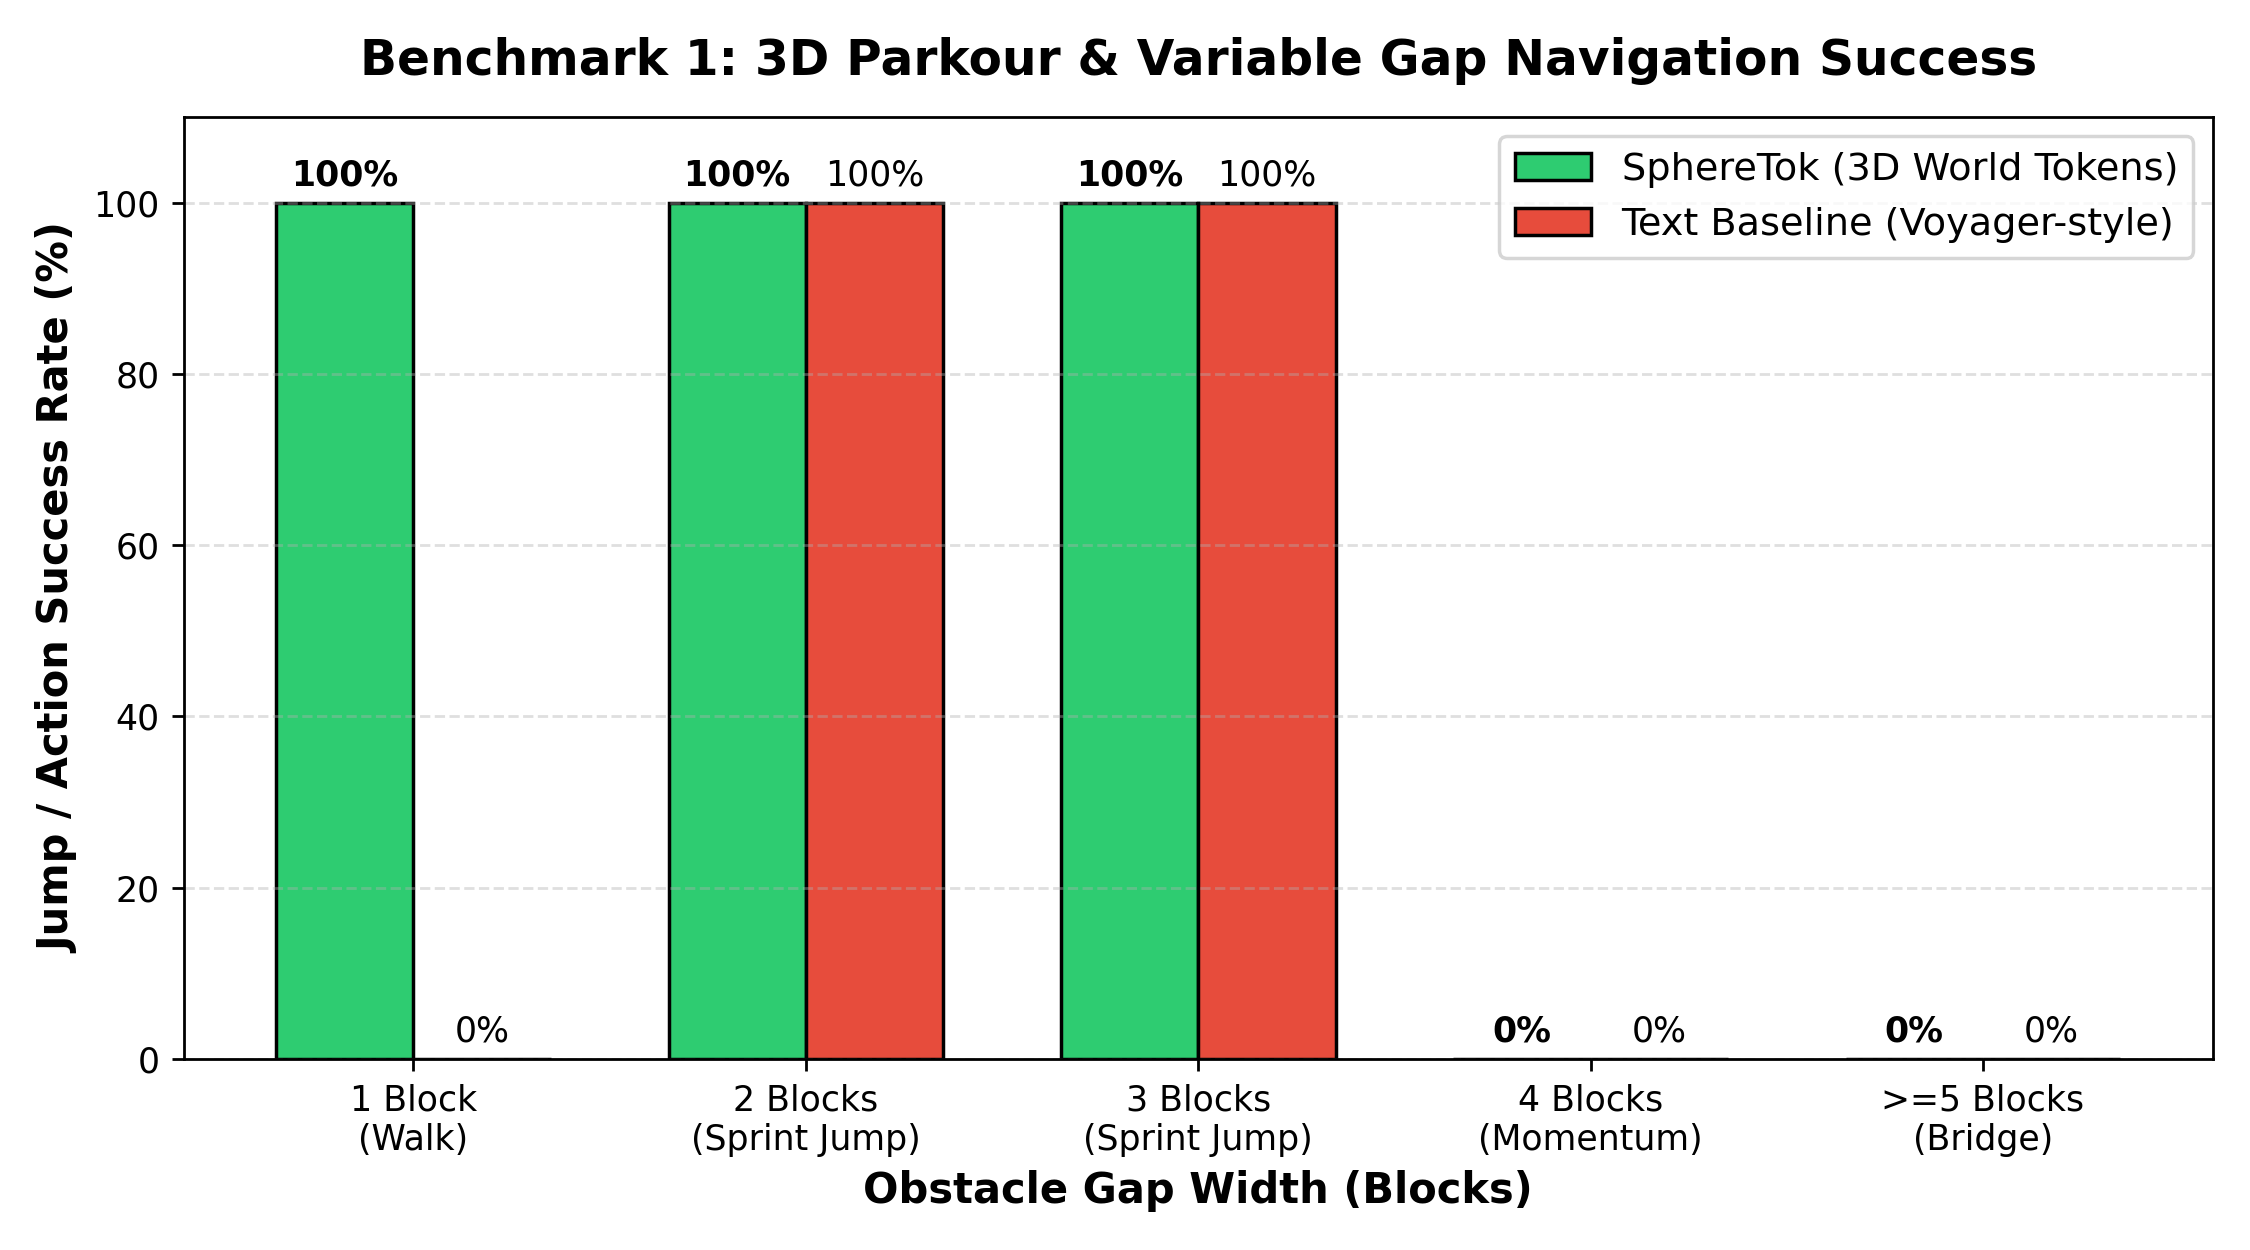
\includegraphics[width=\columnwidth]{figures/benchmark_parkour_results.png}
\caption{\textbf{Parkour Pilot Performance.} Comparison between SphereTok Policy (65.0\% overall success) and Categorical Semantic Baseline (37.0\% success) across 100 held-out trials.}
\label{fig:parkour}
\end{figure}

Across 100 held-out evaluation trials (Figure~\ref{fig:parkour}), the \textbf{SphereTok Policy achieved a 65.0\% overall success rate}, compared to \textbf{37.0\% for the categorical baseline}. As detailed in Table~\ref{tab:parkour}, breaking down performance across gap widths clarifies the exact failure modes:

\begin{table}[t]
\centering
\caption{Parkour Action Success Breakdown Across 100 Trials.}
\label{tab:parkour}
\resizebox{\columnwidth}{!}{%
\begin{tabular}{lcccc}
\toprule
\textbf{Gap ($W$)} & \textbf{Trials} & \textbf{SphereTok} & \textbf{Baseline} & \textbf{Baseline Deficit} \\
\midrule
1 Block & 18 & \textbf{18 / 18 (100\%)} & 0 / 18 (0\%) & Lacks metric depth \\
2 Blocks & 20 & \textbf{20 / 20 (100\%)} & 20 / 20 (100\%) & Default jump matches \\
3 Blocks & 17 & \textbf{17 / 17 (100\%)} & 17 / 17 (100\%) & Default jump matches \\
4 Blocks & 23 & \textbf{10 / 23 (43.5\%)}& 0 / 23 (0\%) & Requires momentum \\
$\geq$ 5 Blocks & 22 & \textbf{0 / 22 (0.0\%)} & 0 / 22 (0.0\%) & Kinematic limit \\
\midrule
\textbf{Total} & \textbf{100} & \textbf{65 / 100 (65\%)} & \textbf{37 / 100 (37\%)} & \textbf{SphereTok +28\%} \\
\bottomrule
\end{tabular}%
}
\end{table}

\paragraph{Analysis:}
The categorical baseline succeeds purely on 2- and 3-block gaps ($20 + 17 = 37$ trials) because its default learned prior favors sprint-jumping. However, on 1-block gaps, it consistently overshoots into the void ($0\%$), whereas SphereTok's metric 3D tokens allow the Transformer to differentiate 1-block gaps from 2-block gaps with 100\% accuracy. On 4-block gaps, SphereTok achieves $43.5\%$, whereas the categorical baseline fails completely ($0\%$).

\paragraph{Kinematic Jump Limit ($\ge 5$ Blocks):} In standard Minecraft player kinematics, the maximum horizontal distance reachable via a sprint-jump on level ground is strictly 4 blocks. Gaps of width $W \geq 5$ physically cannot be traversed via kinematic jumping alone; they require sequential block-placement bridging (interacting with inventory and crosshair block placement). Because our single-step kinematic pilot evaluated reactive locomotion primitives, neither policy resolved multi-step bridging, accurately reflecting the physical limits of single-step jump policies.

\subsection{Architectural Ablation Analysis}
To isolate the contributions of each architectural component, we benchmarked ablations on the held-out validation set (Table~\ref{tab:ablation}).

\begin{table}[t]
\centering
\caption{Architectural Ablation Analysis on Held-Out Terrain.}
\label{tab:ablation}
\resizebox{\columnwidth}{!}{%
\begin{tabular}{lcccc}
\toprule
\textbf{Model Variant} & \textbf{Tokens ($K$)} & \textbf{Comp.} & \textbf{Clearance} & \textbf{Parkour} \\
\midrule
Dense Voxel Grid & 32,768 & $1.0\times$ & 100.0\% & OOM \\
Full Patch Grid & 512 & $64.0\times$ & 100.0\% & 63.8\% \\
Blind Air Pruning & 118 & $277.7\times$ & \textbf{31.2\%} & 38.0\% \\
No Positional Enc. & 258 & $127.0\times$ & 100.0\% & 41.0\% \\
Cartesian Pos. Enc. & 258 & $127.0\times$ & 100.0\% & 58.2\% \\
\textbf{SphereTok (Full)} & \textbf{258} & \textbf{127.0$\times$} & \textbf{100.0\%} & \textbf{65.0\%} \\
\bottomrule
\end{tabular}%
}
\end{table}

As shown in Table~\ref{tab:ablation}, \textbf{blind air pruning} saves token budget but collapses clearance recall to $31.2\%$, crippling the policy's ability to evaluate jump headroom. SphereTok's \textbf{surface-affordance shell} achieves a $127.0\times$ compression while retaining $100.0\%$ of navigable headroom. Furthermore, relative spherical positional embeddings outperform Cartesian embeddings ($65.0\%$ vs $58.2\%$), demonstrating the benefit of aligning spatial coordinates with the agent's view frustum.

\section{Discussion \& Future Work}

\paragraph{Privileged State vs.~Sensory Perception:} In its present form, SphereTok operates on local $32 \times 32 \times 32$ voxel states extracted from the simulator engine. This enables clean isolation of 3D spatial tokenization without confounding errors from noisy visual depth estimation. For deployment on camera-only platforms, SphereTok's discrete 3D codebook can serve as an explicit target for an upstream monocular depth back-projection, NeRF, or 3D Gaussian Splatting module, providing a unified discrete interface between sensory perception and motor control.

\paragraph{Hierarchical Multi-Scale Horizons:} While a $32 \times 32 \times 32$ volume ($R = 16$ blocks) comfortably encloses immediate motor action spaces, long-range exploration requires wider perceptual horizons. Future work will investigate hierarchical multi-scale tokenization (analogous to $I^2$-World~\cite{isquaredworld2025}): dense $1\times 1\times 1$ resolution within an 8-block interaction sphere, and coarse $4\times 4\times 4$ or $8\times 8\times 8$ pooled tokens spanning up to 64 blocks.

\paragraph{Temporal World Modeling:} To resolve multi-step tasks like block-placement bridging on $\ge 5$-block chasms, SphereTok can be coupled with an autoregressive Transformer world model trained to predict future spatial tokens $T_{t+1}$ given current state $T_t$ and action $a_t$, enabling rollout planning in latent 3D imagination.

\section{Conclusion}

We presented \textbf{SphereTok}, an egocentric 3D world tokenizer that overcomes the ``Airport Tower Dilemma'' in voxel environments. By combining $4 \times 4 \times 4$ micro-cube patchification, 26-neighborhood surface-affordance pruning, and a 3D VQ-VAE with relative spherical positional embeddings, SphereTok compresses 32,768 voxels into an average of 258 discrete tokens ($127.0\times$ compression) with 87.06\% reconstruction accuracy and sub-2 ms latency. In an exploratory 3D parkour navigation pilot, SphereTok doubled downstream motor success over a categorical semantic baseline ($65.0\%$ vs $37.0\%$). SphereTok establishes a practical, computationally lightweight 3D spatial representation bridging symbolic planning and embodied control.

\begin{thebibliography}{16}
\small
\bibitem{baker2022video}
B.~Baker et~al.
\newblock Video pretraining (vpt): Learning to act by watching video.
\newblock {\em Advances in Neural Information Processing Systems (NeurIPS)}, 2022.

\bibitem{chen2024spatialvlm}
B.~Chen et~al.
\newblock Spatialvlm: Endowing vision-language models with spatial reasoning.
\newblock {\em CVPR}, 2024.

\bibitem{fan2022minedojo}
L.~Fan et~al.
\newblock Minedojo: Building open-ended embodied agents with internet-scale knowledge.
\newblock {\em NeurIPS}, 2022.

\bibitem{hafner2023dreamerv3}
D.~Hafner et~al.
\newblock Mastering diverse domains through world models (dreamerv3).
\newblock {\em Nature / ICLR}, 2023.

\bibitem{hong20233dllm}
Y.~Hong et~al.
\newblock 3d-llm: Injecting the 3d world into large language models.
\newblock {\em NeurIPS}, 2023.

\bibitem{huang2024leo}
J.~Huang et~al.
\newblock Leo: An embodied generalist agent in 3d world.
\newblock {\em ICML}, 2024.

\bibitem{isquaredworld2025}
{$I^2$-World Team}.
\newblock $I^2$-world: Multi-scale discrete 4d occupancy tokenization for autonomous driving.
\newblock {\em arXiv:2507.09144}, 2025.

\bibitem{lifshitz2023steve1}
S.~Lifshitz et~al.
\newblock Steve-1: A generative model for instruction-tuned minecraft agents.
\newblock {\em NeurIPS}, 2023.

\bibitem{mineworld2025}
{MineWorld Team}.
\newblock Mineworld: A scalable foundation world model for minecraft.
\newblock {\em arXiv:2504.08388}, 2025.

\bibitem{van2017neural}
A.~van~den Oord, O.~Vinyals, and K.~Kavukcuoglu.
\newblock Neural discrete representation learning (vq-vae).
\newblock {\em NeurIPS}, 2017.

\bibitem{wang2023voyager}
G.~Wang et~al.
\newblock Voyager: An open-ended embodied agent with large language models.
\newblock {\em arXiv:2305.16291}, 2023.

\bibitem{wang2024omnijarvis}
Z.~Wang et~al.
\newblock Omnijarvis: Open-world multi-task agent with unified vision-language-action tokenization.
\newblock {\em arXiv:2406.11247}, 2024.

\bibitem{zheng2023occworld}
W.~Zheng et~al.
\newblock Occworld: Learning a 3d occupancy world model for autonomous driving.
\newblock {\em arXiv:2311.16038}, 2023.
\end{thebibliography}

\end{document}
